% =====================================================================
% Numerical Linear Algebra -- Project 5: Low-Rank Approximation
% Authors: Abhishek Jha, Favour Gilbert, Shehaan Butt
% Compile with: pdflatex main.tex   (requires TikZ + pgfplots)
% =====================================================================
\documentclass[10pt,aspectratio=169]{beamer}

\usetheme{metropolis}
\usecolortheme{orchid}
\setbeamertemplate{navigation symbols}{}
\setbeamertemplate{caption}[numbered]

\usepackage{amsmath, amssymb, amsthm}
\usepackage{mathtools}
\usepackage{tikz}
\usepackage{pgfplots}
\pgfplotsset{compat=1.18}
\usetikzlibrary{arrows.meta, positioning, decorations.pathreplacing, calc, shapes.geometric}
\usepackage{graphicx}
\usepackage{booktabs}
\usepackage{xcolor}

% Tell graphicx where to look for figures
\graphicspath{{figs/}}

% --- Math shortcuts ---
\DeclareMathOperator{\rank}{rank}
\DeclareMathOperator{\tr}{tr}
\newcommand{\R}{\mathbb{R}}
\newcommand{\norm}[1]{\left\|#1\right\|}

% --- Title ---
\title[Low-Rank Approximation]{Low-Rank Approximation}
\author[Jha \and Gilbert \and Butt]{
  Abhishek Jha \and Favour Gilbert Mmesoma \and Muhammad Shehaan Butt
}
\institute[Uni.lu]{MSc Mathematical Modelling and Computational Sciences\\
University of Luxembourg}
\date{\today}

% Section pages
\AtBeginSection[]{
  \begin{frame}{Outline}
    \tableofcontents[currentsection, sectionstyle=show/shaded]
  \end{frame}
}

\begin{document}

% =====================================================================
\begin{frame}
  \titlepage
\end{frame}

\begin{frame}{Outline}
  \tableofcontents
\end{frame}

% =====================================================================
\section{Motivation}
% =====================================================================

\begin{frame}{Why Low-Rank Approximation?}
  Modern matrices are \emph{huge} but their information content is often \emph{small}.
  \begin{itemize}
    \item A single HD image: $\sim$$10^6$ pixels, but neighbouring pixels are highly correlated.
    \item A user--movie ratings matrix: millions of rows and columns, $99\%+$ unobserved.
    \item Gene-expression data: $20{,}000$ genes per sample, but only a handful of biological pathways drive the variance.
  \end{itemize}
  In each case, the \emph{effective} rank is far smaller than the apparent size of the matrix. Low-rank approximation lets us:
  \begin{itemize}
    \item store and transmit data with far fewer numbers,
    \item reveal latent structure (principal components, topics, communities),
    \item separate \emph{signal} (large singular values) from \emph{noise} (small ones).
  \end{itemize}
\end{frame}

\begin{frame}{The Problem We Are Solving}
  Given $A \in \R^{m\times n}$ and a target rank $k \ll \min(m,n)$, find
  \[
    B^\star \;=\; \arg\min_{B:\, \rank(B) \le k} \norm{A - B}.
  \]
  Two questions arise:
  \begin{enumerate}
    \item Which norm? -- different choices give different optima.
    \item How do we compute $B^\star$ in practice?
  \end{enumerate}
  \medskip
  \textbf{Spoiler.} For both the Frobenius and the spectral norm, the answer is given by the \emph{truncated singular value decomposition} (Eckart--Young--Mirsky theorem). The proof and its consequences form the spine of this talk.
\end{frame}

\begin{frame}{What This Project Covers}
  \textbf{Theory.}
  \begin{itemize}
    \item Matrix norms (Frobenius, spectral) and unitary invariance.
    \item Singular value decomposition: existence, geometry, link to eigendecomposition.
    \item Truncated SVD and the Eckart--Young--Mirsky theorem (full proof).
    \item Singular value decay and the notion of numerical rank.
  \end{itemize}
  \textbf{Applications.}
  \begin{itemize}
    \item \textbf{Image compression} via truncated SVD -- compression, denoising.
    \item \textbf{PCA on MNIST} -- dimensionality reduction.
  \end{itemize}
  \textbf{Deliverables.}
  \begin{itemize}
    \item Two Jupyter notebooks (one per application).
    \item Two interactive Streamlit web apps.
    \item This presentation.
  \end{itemize}
\end{frame}

% =====================================================================
\section{Matrix Norms}
% =====================================================================

\begin{frame}{Frobenius Norm}
  \begin{block}{Definition}
    For $A \in \R^{m \times n}$,
    \[
      \norm{A}_F \;=\; \sqrt{\sum_{i=1}^m \sum_{j=1}^n |a_{ij}|^2}
                 \;=\; \sqrt{\tr(A^\top A)}.
    \]
  \end{block}
  \begin{itemize}
    \item Euclidean norm of $A$ regarded as a vector in $\R^{mn}$.
    \item In singular values: $\norm{A}_F = \sqrt{\sum_{i=1}^{r} \sigma_i^2}$.
    \item Easy to compute, smooth, induced by the Frobenius inner product
      $\langle A, B\rangle_F = \tr(A^\top B)$.
    \item \textbf{Interpretation.} Aggregates error \emph{uniformly} across all entries -- a small Frobenius error means the matrices are close \emph{on average}.
  \end{itemize}
\end{frame}

\begin{frame}{Spectral Norm (Operator 2-Norm)}
  \begin{block}{Definition}
    \[
      \norm{A}_2 \;=\; \sup_{x \neq 0} \frac{\norm{Ax}_2}{\norm{x}_2}
                 \;=\; \sigma_1(A).
    \]
  \end{block}
  \begin{itemize}
    \item Largest singular value: maximum stretching factor on the unit ball.
    \item Captures \emph{worst-case} amplification, unlike $\norm{\cdot}_F$ which is an aggregate.
    \item Geometrically: $A$ maps the unit ball to an ellipsoid; $\norm{A}_2$ is the longest semi-axis.
  \end{itemize}

  \vspace{0.3cm}
  \begin{center}
    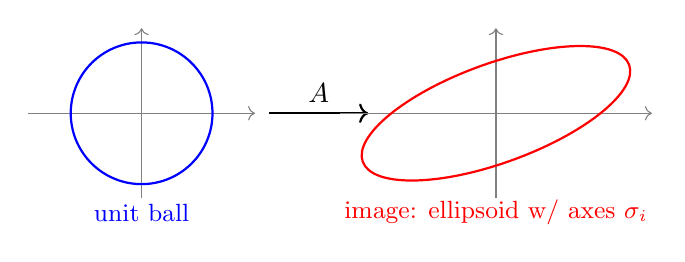
\begin{tikzpicture}[scale=0.9]
      \draw[->, gray] (-1.6,0) -- (1.6,0);
      \draw[->, gray] (0,-1.2) -- (0,1.2);
      \draw[blue, thick] (0,0) circle (1);
      \node[blue] at (0,-1.4) {\small unit ball};

      \draw[->, thick] (1.8,0) -- (3.2,0) node[midway, above] {$A$};

      \begin{scope}[xshift=5cm]
        \draw[->, gray] (-2.2,0) -- (2.2,0);
        \draw[->, gray] (0,-1.2) -- (0,1.2);
        \draw[red, thick, rotate=20] (0,0) ellipse (2 and 0.7);
        \node[red] at (0,-1.4) {\small image: ellipsoid w/ axes $\sigma_i$};
      \end{scope}
    \end{tikzpicture}
  \end{center}
\end{frame}

\begin{frame}{Unitary Invariance}
  \begin{theorem}
    If $U \in \R^{m\times m}$ and $V \in \R^{n\times n}$ are orthogonal, then
    \[
      \norm{UAV}_F = \norm{A}_F, \qquad \norm{UAV}_2 = \norm{A}_2.
    \]
  \end{theorem}
  \emph{Idea.} Orthogonal matrices preserve lengths and angles; multiplying by them only rotates / reflects, never stretches. Both norms see only the singular values, which are invariant under such rotations.

  \begin{proof}[Proof (Frobenius)]
    Use $\norm{M}_F^2 = \tr(M^\top M)$ and the fact that $U^\top U = I$:
    \[
      \norm{UA}_F^2 = \tr(A^\top U^\top U A) = \tr(A^\top A) = \norm{A}_F^2.
    \]
    Right-multiplication: $\norm{AV}_F^2 = \tr(V^\top A^\top A V) = \tr(A^\top A)$ by cyclicity of trace.
  \end{proof}
  \begin{proof}[Proof (Spectral)]
    Lengths: $\norm{UAVx}_2 = \norm{AVx}_2$ since $U$ is orthogonal. As $x$ ranges over the unit sphere, so does $Vx$ (orthogonal map). Hence the supremum is unchanged.
  \end{proof}
\end{frame}

\begin{frame}{Why Unitary Invariance Matters}
  Both norms depend \emph{only} on the singular values:
  \[
    \norm{A}_F = \sqrt{\textstyle\sum_i \sigma_i^2}, \qquad \norm{A}_2 = \sigma_1.
  \]

  \begin{block}{Consequence (used repeatedly later)}
    When proving optimality of low-rank approximations we may freely rotate the coordinate system -- specifically, we can pre-multiply by $U^\top$ and post-multiply by $V$ to bring $A$ into the diagonal form $\Sigma$ \emph{without changing any norms}. This converts a hard matrix optimisation into a simple statement about singular values.
  \end{block}
\end{frame}

% =====================================================================
\section{Singular Value Decomposition}
% =====================================================================

\begin{frame}{The Theorem}
  \begin{theorem}[SVD]
    Every $A \in \R^{m \times n}$ admits a factorisation
    \[
      A \;=\; U\,\Sigma\,V^\top,
    \]
    with
    \begin{itemize}
      \item $U \in \R^{m\times m}$, $V \in \R^{n\times n}$ orthogonal,
      \item $\Sigma \in \R^{m\times n}$ diagonal with entries
        $\sigma_1 \geq \sigma_2 \geq \cdots \geq \sigma_r > 0 = \sigma_{r+1} = \cdots,$
      \item $r = \rank(A)$.
    \end{itemize}
  \end{theorem}
  Columns $u_i$ of $U$: \emph{left} singular vectors. Columns $v_i$ of $V$: \emph{right} singular vectors.\\
  \medskip
  The SVD always exists -- unlike the eigendecomposition, which requires $A$ to be square and diagonalisable.
\end{frame}

\begin{frame}{Geometric Interpretation}
  $A$ acts as: \textbf{rotate} $V^\top$ $\to$ \textbf{stretch} $\Sigma$ $\to$ \textbf{rotate} $U$.

  \vspace{0.4cm}
  \begin{center}
    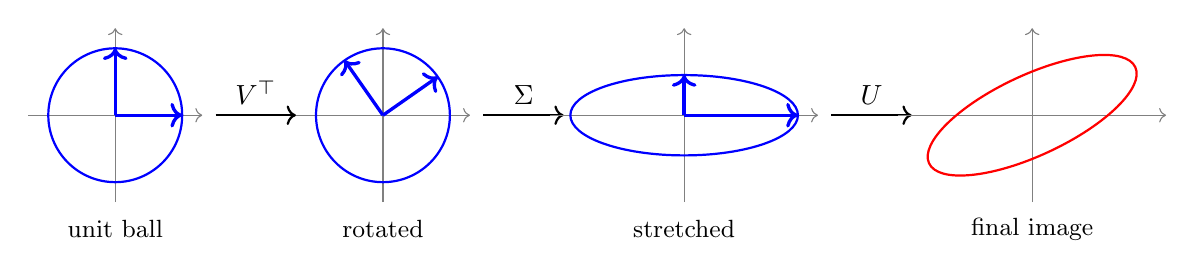
\begin{tikzpicture}[scale=0.85]
      % Stage 1: unit circle
      \draw[->, gray] (-1.3,0) -- (1.3,0);
      \draw[->, gray] (0,-1.3) -- (0,1.3);
      \draw[blue, thick] (0,0) circle (1);
      \draw[->, very thick, blue] (0,0) -- (1,0);
      \draw[->, very thick, blue] (0,0) -- (0,1);
      \node at (0,-1.7) {\small unit ball};

      \draw[->, thick] (1.5,0) -- (2.7,0) node[midway, above] {$V^\top$};

      % Stage 2: rotated
      \begin{scope}[xshift=4cm]
        \draw[->, gray] (-1.3,0) -- (1.3,0);
        \draw[->, gray] (0,-1.3) -- (0,1.3);
        \draw[blue, thick] (0,0) circle (1);
        \draw[->, very thick, blue, rotate=35] (0,0) -- (1,0);
        \draw[->, very thick, blue, rotate=35] (0,0) -- (0,1);
        \node at (0,-1.7) {\small rotated};
      \end{scope}

      \draw[->, thick] (5.5,0) -- (6.7,0) node[midway, above] {$\Sigma$};

      % Stage 3: scaled (ellipse)
      \begin{scope}[xshift=8.5cm]
        \draw[->, gray] (-2,0) -- (2,0);
        \draw[->, gray] (0,-1.3) -- (0,1.3);
        \draw[blue, thick] (0,0) ellipse (1.7 and 0.6);
        \draw[->, very thick, blue] (0,0) -- (1.7,0);
        \draw[->, very thick, blue] (0,0) -- (0,0.6);
        \node at (0,-1.7) {\small stretched};
      \end{scope}

      \draw[->, thick] (10.7,0) -- (11.9,0) node[midway, above] {$U$};

      % Stage 4: rotated ellipse
      \begin{scope}[xshift=13.7cm]
        \draw[->, gray] (-2,0) -- (2,0);
        \draw[->, gray] (0,-1.3) -- (0,1.3);
        \draw[red, thick, rotate=25] (0,0) ellipse (1.7 and 0.6);
        \node at (0,-1.7) {\small final image};
      \end{scope}
    \end{tikzpicture}
  \end{center}
  Every linear map factors into rotation--stretch--rotation. The stretch factors are the singular values, and the directions of stretch are the columns of $V$ (input) and $U$ (output).
\end{frame}

\begin{frame}{Existence: Constructive Proof}
  \emph{Strategy.} Build $V$ from the spectral theorem applied to $A^\top A$, define singular values as square roots of its eigenvalues, then construct $U$ so that $A = U\Sigma V^\top$ falls out.
  \begin{enumerate}
    \item $A^\top A \in \R^{n\times n}$ is symmetric positive semidefinite, hence has non-negative real eigenvalues.
    \item Spectral theorem: $A^\top A = V \Lambda V^\top$ with $\Lambda = \mathrm{diag}(\lambda_1 \geq \cdots \geq \lambda_n \geq 0)$ and $V$ orthogonal.
    \item Set $\sigma_i = \sqrt{\lambda_i}$ and, for $\sigma_i > 0$, $u_i = \dfrac{Av_i}{\sigma_i}$.
    \item Check orthonormality of $\{u_i\}$:
      \[
        u_i^\top u_j = \frac{v_i^\top A^\top A v_j}{\sigma_i \sigma_j} = \frac{\lambda_j}{\sigma_i \sigma_j} v_i^\top v_j = \delta_{ij}.
      \]
    \item Extend $\{u_1,\dots,u_r\}$ to an orthonormal basis of $\R^m$ (Gram--Schmidt).
    \item By construction $A v_j = \sigma_j u_j$, so $AV = U\Sigma$, i.e.\ $A = U \Sigma V^\top$. \qed
  \end{enumerate}
\end{frame}

\begin{frame}{Connection to Eigendecomposition}
  \begin{itemize}
    \item $A^\top A = V \Sigma^\top \Sigma V^\top$:\\
      right singular vectors $=$ eigenvectors of $A^\top A$,\quad eigenvalues $= \sigma_i^2$.
    \item $A A^\top = U \Sigma \Sigma^\top U^\top$:\\
      left singular vectors $=$ eigenvectors of $A A^\top$.
    \item For symmetric $A \succeq 0$: SVD $\equiv$ eigendecomposition.
    \item For symmetric $A$ with negative eigenvalues: $\sigma_i = |\lambda_i|$, sign absorbed into $U$.
    \item \textbf{Numerical caution.} Forming $A^\top A$ explicitly squares the condition number. Production solvers (LAPACK \texttt{gesvd}, \texttt{gesdd}) bypass this with bidiagonalisation followed by implicit-shift QR.
  \end{itemize}
\end{frame}

% =====================================================================
\section{Truncated SVD}
% =====================================================================

\begin{frame}{Rank-$k$ Approximation}
  Outer-product form of the SVD:
  \[
    A \;=\; \sum_{i=1}^{r} \sigma_i\, u_i v_i^\top.
  \]
  Each term $\sigma_i u_i v_i^\top$ is a rank-1 matrix; the SVD writes $A$ as a sum of $r$ such ``elementary'' pieces, ordered by importance.

  \medskip
  The \emph{truncated SVD} of order $k \leq r$ keeps only the leading $k$ terms:
  \[
    A_k \;=\; \sum_{i=1}^{k} \sigma_i\, u_i v_i^\top \;=\; U_k \Sigma_k V_k^\top.
  \]
  \begin{itemize}
    \item $U_k \in \R^{m\times k}$, $\Sigma_k \in \R^{k\times k}$, $V_k \in \R^{n\times k}$.
    \item $\rank(A_k) = k$.
  \end{itemize}
\end{frame}

\begin{frame}{Outer-Product Picture}
  \begin{center}
    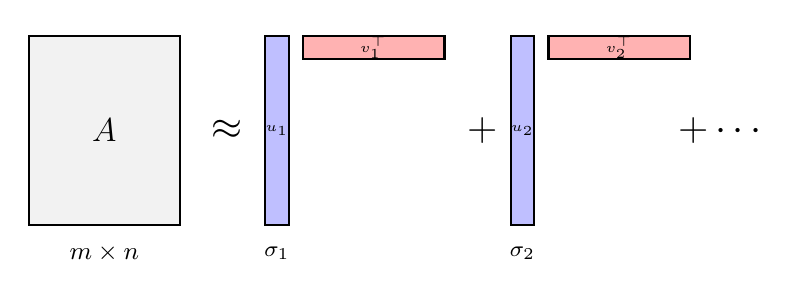
\begin{tikzpicture}[scale=0.6]
      % A
      \draw[thick, fill=gray!10] (0,0) rectangle (3.2,4);
      \node at (1.6,2) {\large $A$};
      \node at (1.6,-0.6) {\small $m\times n$};

      \node at (4.2,2) {\Large $\approx$};

      % term 1
      \draw[thick, fill=blue!25] (5,0) rectangle (5.5,4); \node at (5.25,2) {\tiny $u_1$};
      \draw[thick, fill=red!30] (5.8,3.5) rectangle (8.8,4); \node at (7.3,3.75) {\tiny $v_1^\top$};
      \node at (5.25,-0.6) {\footnotesize $\sigma_1$};

      \node at (9.6,2) {\Large $+$};

      % term 2
      \draw[thick, fill=blue!25] (10.2,0) rectangle (10.7,4); \node at (10.45,2) {\tiny $u_2$};
      \draw[thick, fill=red!30] (11,3.5) rectangle (14,4); \node at (12.5,3.75) {\tiny $v_2^\top$};
      \node at (10.45,-0.6) {\footnotesize $\sigma_2$};

      \node at (14.7,2) {\Large $+ \cdots$};
    \end{tikzpicture}
  \end{center}
  \vspace{0.3cm}
  Each rank-1 term costs $m + n$ numbers + 1 scalar -- truncating to $k$ terms gives storage $k(m+n+1)$ instead of $mn$.
\end{frame}

\begin{frame}{Compact Storage}
  \begin{itemize}
    \item Full $A$: $mn$ entries.
    \item $A_k$ stored as $(U_k, \Sigma_k, V_k)$:\quad $k(m + n + 1)$ numbers.
    \item Compression whenever $k(m+n+1) \ll mn$, i.e.\ $k \ll \dfrac{mn}{m+n+1}$.
  \end{itemize}

  \begin{block}{Example: $1024 \times 1024$ image}
    \begin{tabular}{lrr}
      \toprule
      $k$ & storage (numbers) & ratio \\
      \midrule
      full     & $1{,}048{,}576$ & 1.00 \\
      $k=100$  & $204{,}900$     & 0.20 \\
      $k=50$   & $102{,}450$     & 0.10 \\
      $k=20$   & $40{,}980$      & 0.04 \\
      \bottomrule
    \end{tabular}
  \end{block}
\end{frame}

% =====================================================================
\section{Eckart--Young--Mirsky Theorem}
% =====================================================================

\begin{frame}{Statement}
  \begin{theorem}[Eckart--Young--Mirsky]
    Let $A \in \R^{m\times n}$ with SVD $A = U\Sigma V^\top$, and $A_k$ its rank-$k$ truncation. Then:
    \[
      \min_{\rank(B) \leq k} \norm{A-B}_2 \;=\; \norm{A-A_k}_2 \;=\; \sigma_{k+1},
    \]
    \[
      \min_{\rank(B) \leq k} \norm{A-B}_F \;=\; \norm{A-A_k}_F \;=\; \sqrt{\sum_{i=k+1}^{r} \sigma_i^2}.
    \]
  \end{theorem}
  Truncated SVD is \emph{the} optimal low-rank approximation in both norms. The error has a closed form -- computing $A_k$ and reading off the leftover singular values immediately tells us how good the approximation is.
\end{frame}

\begin{frame}{Proof (Spectral Norm) -- Step 1: Upper Bound}
  \emph{Goal.} Show that the truncation error itself is small -- specifically, $\sigma_{k+1}$. This gives an \emph{achievable} value, hence an upper bound on the minimum.

  \medskip
  Compute the residual directly from the outer-product expansion:
  \[
    A - A_k = \sum_{i=k+1}^{r} \sigma_i\, u_i v_i^\top.
  \]
  This is itself an SVD-shaped sum, with singular values $\sigma_{k+1}, \sigma_{k+2}, \ldots$. Since the spectral norm equals the largest singular value:
  \[
    \norm{A - A_k}_2 = \sigma_{k+1}.
  \]
  Therefore $\displaystyle \min_{\rank(B)\leq k} \norm{A - B}_2 \leq \sigma_{k+1}$ -- the truncated SVD achieves at most this error.
\end{frame}

\begin{frame}{Proof (Spectral Norm) -- Step 2: Lower Bound}
  \emph{Strategy.} Show that no rank-$k$ matrix can do \emph{better}. Trick: find a vector $w$ that is killed by $B$ but stretched a lot by $A$. Then $\norm{(A-B)w} = \norm{Aw}$ is large, forcing $\norm{A-B}_2$ to be large.
  \medskip

  Let $B$ be any matrix with $\rank(B) \leq k$. By rank-nullity, $\dim \ker(B) \geq n - k$.

  \medskip
  Consider $W = \mathrm{span}\{v_1, \dots, v_{k+1}\}$, a $(k+1)$-dimensional subspace.

  \medskip
  Two subspaces of $\R^n$, of dimensions $\geq n-k$ and $k+1$, must intersect non-trivially:
  \[
    \dim(\ker B \cap W) \;\geq\; (n-k) + (k+1) - n \;=\; 1.
  \]
  Pick a unit vector $w \in \ker B \cap W$, write $w = \sum_{i=1}^{k+1} \alpha_i v_i$ with $\sum \alpha_i^2 = 1$.
\end{frame}

\begin{frame}{Proof (Spectral Norm) -- Step 3: Conclude}
  Since $Bw = 0$, the action of $B$ on $w$ vanishes:
  \[
    \norm{A - B}_2^2 \;\geq\; \norm{(A-B)w}_2^2 \;=\; \norm{Aw}_2^2.
  \]
  Now compute $\norm{Aw}_2^2$ using $A v_i = \sigma_i u_i$ and orthonormality of $\{u_i\}$:
  \[
    \norm{Aw}_2^2 = \norm{\sum_{i=1}^{k+1} \alpha_i \sigma_i u_i}_2^2 = \sum_{i=1}^{k+1} \alpha_i^2 \sigma_i^2.
  \]
  Each $\sigma_i \geq \sigma_{k+1}$ for $i \leq k+1$, so
  \[
    \sum_{i=1}^{k+1} \alpha_i^2 \sigma_i^2 \;\geq\; \sigma_{k+1}^2 \sum_{i=1}^{k+1} \alpha_i^2 = \sigma_{k+1}^2.
  \]
  Therefore $\norm{A - B}_2 \geq \sigma_{k+1}$, matching the upper bound. \qed
\end{frame}

\begin{frame}{Proof (Frobenius Norm)}
  \emph{Idea.} The Frobenius norm sums all singular values squared. We need: any rank-$k$ approximation throws away at least the trailing $\sigma_i^2$. Weyl's inequality formalises this.

  \medskip
  \textbf{Key tool} (Weyl's inequality for singular values): if $\rank(B) \leq k$, then
  \[
    \sigma_{i+k}(A) \;\leq\; \sigma_i(A - B) \quad \text{for all } i \geq 1.
  \]
  \emph{Reading.} The $i$-th singular value of the residual is at least the $(i+k)$-th singular value of $A$ -- the rank-$k$ approximation cannot reach singular values past the first $k$.

  \medskip
  Therefore
  \[
    \norm{A - B}_F^2 = \sum_{i \geq 1} \sigma_i(A-B)^2 \;\geq\; \sum_{i \geq 1} \sigma_{i+k}(A)^2 = \sum_{j > k} \sigma_j(A)^2.
  \]
  Equality is attained at $B = A_k$, since $\norm{A - A_k}_F^2 = \sum_{j > k} \sigma_j^2$. \qed
\end{frame}

% =====================================================================
\section{Singular Value Decay \& Numerical Rank}
% =====================================================================

\begin{frame}{Numerical Rank}
  \begin{itemize}
    \item Real-world matrices rarely have low \emph{exact} rank.
    \item But singular values often decay rapidly $\Rightarrow$ \emph{numerically} low rank.
    \item For tolerance $\varepsilon > 0$:
      \[
        r_\varepsilon \;=\; \#\{ i : \sigma_i > \varepsilon \cdot \sigma_1 \}.
      \]
    \item Eckart--Young--Mirsky gives the exact relative error:
      \[
        \frac{\norm{A - A_k}_F^2}{\norm{A}_F^2} \;=\; \frac{\sum_{i>k}\sigma_i^2}{\sum_i \sigma_i^2}.
      \]
      Fast decay $\Rightarrow$ small relative error at small $k$.
    \item In practice we pick $k$ so that this ratio is below an acceptable threshold (e.g.\ $5\%$, $1\%$).
  \end{itemize}
\end{frame}

\begin{frame}{How is $k$ chosen in practice?}
  \begin{itemize}
    \item \textbf{Design choice:} fix $k$ from a storage / compute budget.
    \item \textbf{Tolerance criterion:} smallest $k$ with relative error $\leq \varepsilon$ (Eckart--Young).
    \item \textbf{Numerical rank:} discard $\sigma_i$ below a noise floor $\tau$.
    \item \textbf{Cross-validation:} when $k$ feeds a downstream task (e.g.\ classification).
    \item \textbf{Optimal threshold (denoising):} closed-form $k^*$ from noise level (Gavish--Donoho).
  \end{itemize}
  $k$ is a knob; what changes is \emph{how we turn it}.
\end{frame}

\begin{frame}{Singular Value Decay (from notebook)}
  \begin{center}
    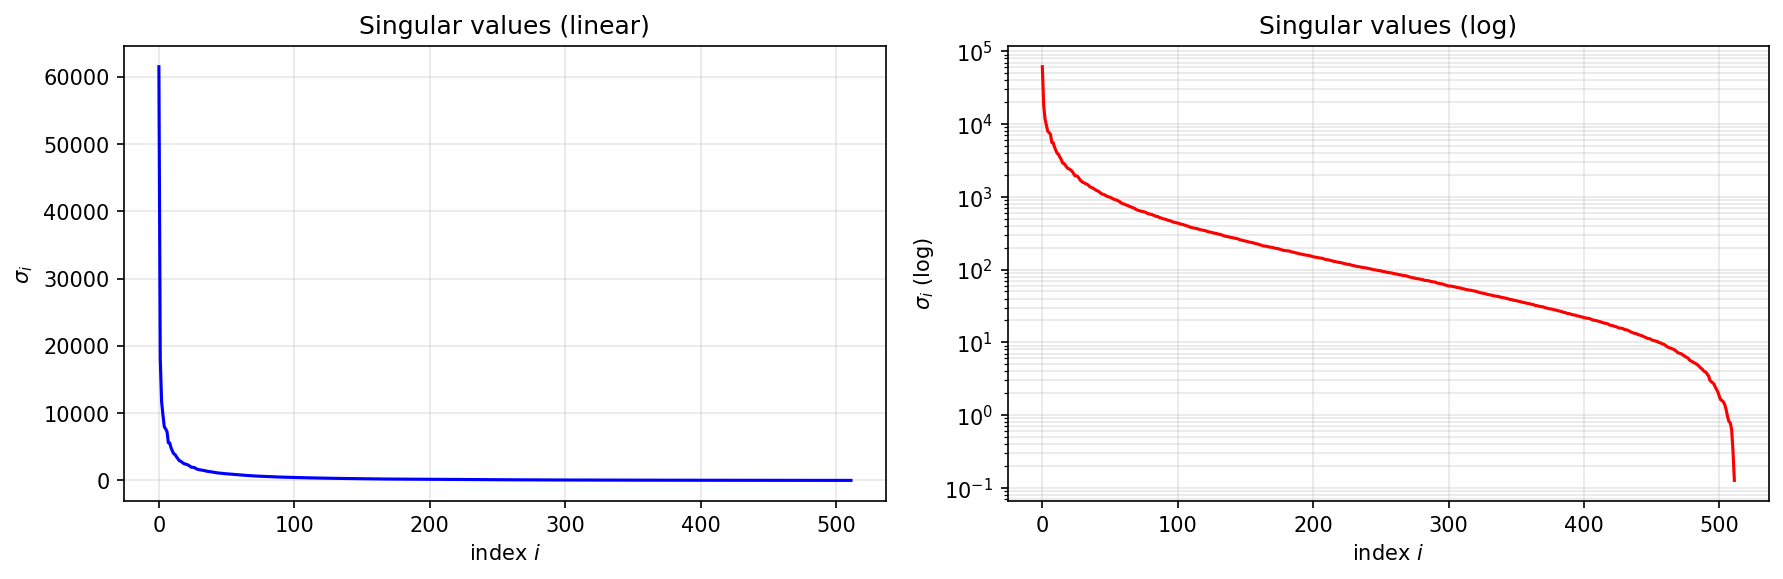
\includegraphics[width=\linewidth,height=0.7\textheight,keepaspectratio]{spectrum.png}
  \end{center}
  \footnotesize \textbf{Observation.} Astronaut image, $512\times 512$. The first singular value is $\sim$$6\times 10^4$; the smallest is $\sim$$10^{-1}$ -- six orders of magnitude of decay. The first 50 components carry essentially all the visual structure; the rest is fine texture and rounding noise.
\end{frame}

% =====================================================================
\section{Application 1: Image Compression}
% =====================================================================

\begin{frame}{Setup}
  \begin{itemize}
    \item Treat a grayscale image as $A \in \R^{m \times n}$ (pixel intensities).
    \item Compute SVD $A = U \Sigma V^\top$.
    \item Reconstruct from rank-$k$ truncation: $A_k = U_k \Sigma_k V_k^\top$.
    \item Vary $k$ to trade off quality vs.\ storage.
    \item Color images: apply per channel (R, G, B treated independently) or stack channels into one tall matrix.
  \end{itemize}
\end{frame}

\begin{frame}{Quality \& Cost Metrics}
  \begin{itemize}
    \item Relative Frobenius error (closed form via Eckart--Young):
      \(
        \dfrac{\norm{A - A_k}_F}{\norm{A}_F}
        = \sqrt{\dfrac{\sum_{i>k} \sigma_i^2}{\sum_i \sigma_i^2}}.
      \)
    \item Compression ratio: $\rho_k = \dfrac{k(m + n + 1)}{mn}$.
    \item PSNR (visual fidelity, dB):
      \(
        \mathrm{PSNR} = 10 \log_{10}\!\dfrac{\mathrm{MAX}^2}{\mathrm{MSE}}.
      \)
      $> 30$ dB is generally considered visually acceptable.
  \end{itemize}
\end{frame}

\begin{frame}{Reconstructions at Increasing $k$}
  \begin{center}
    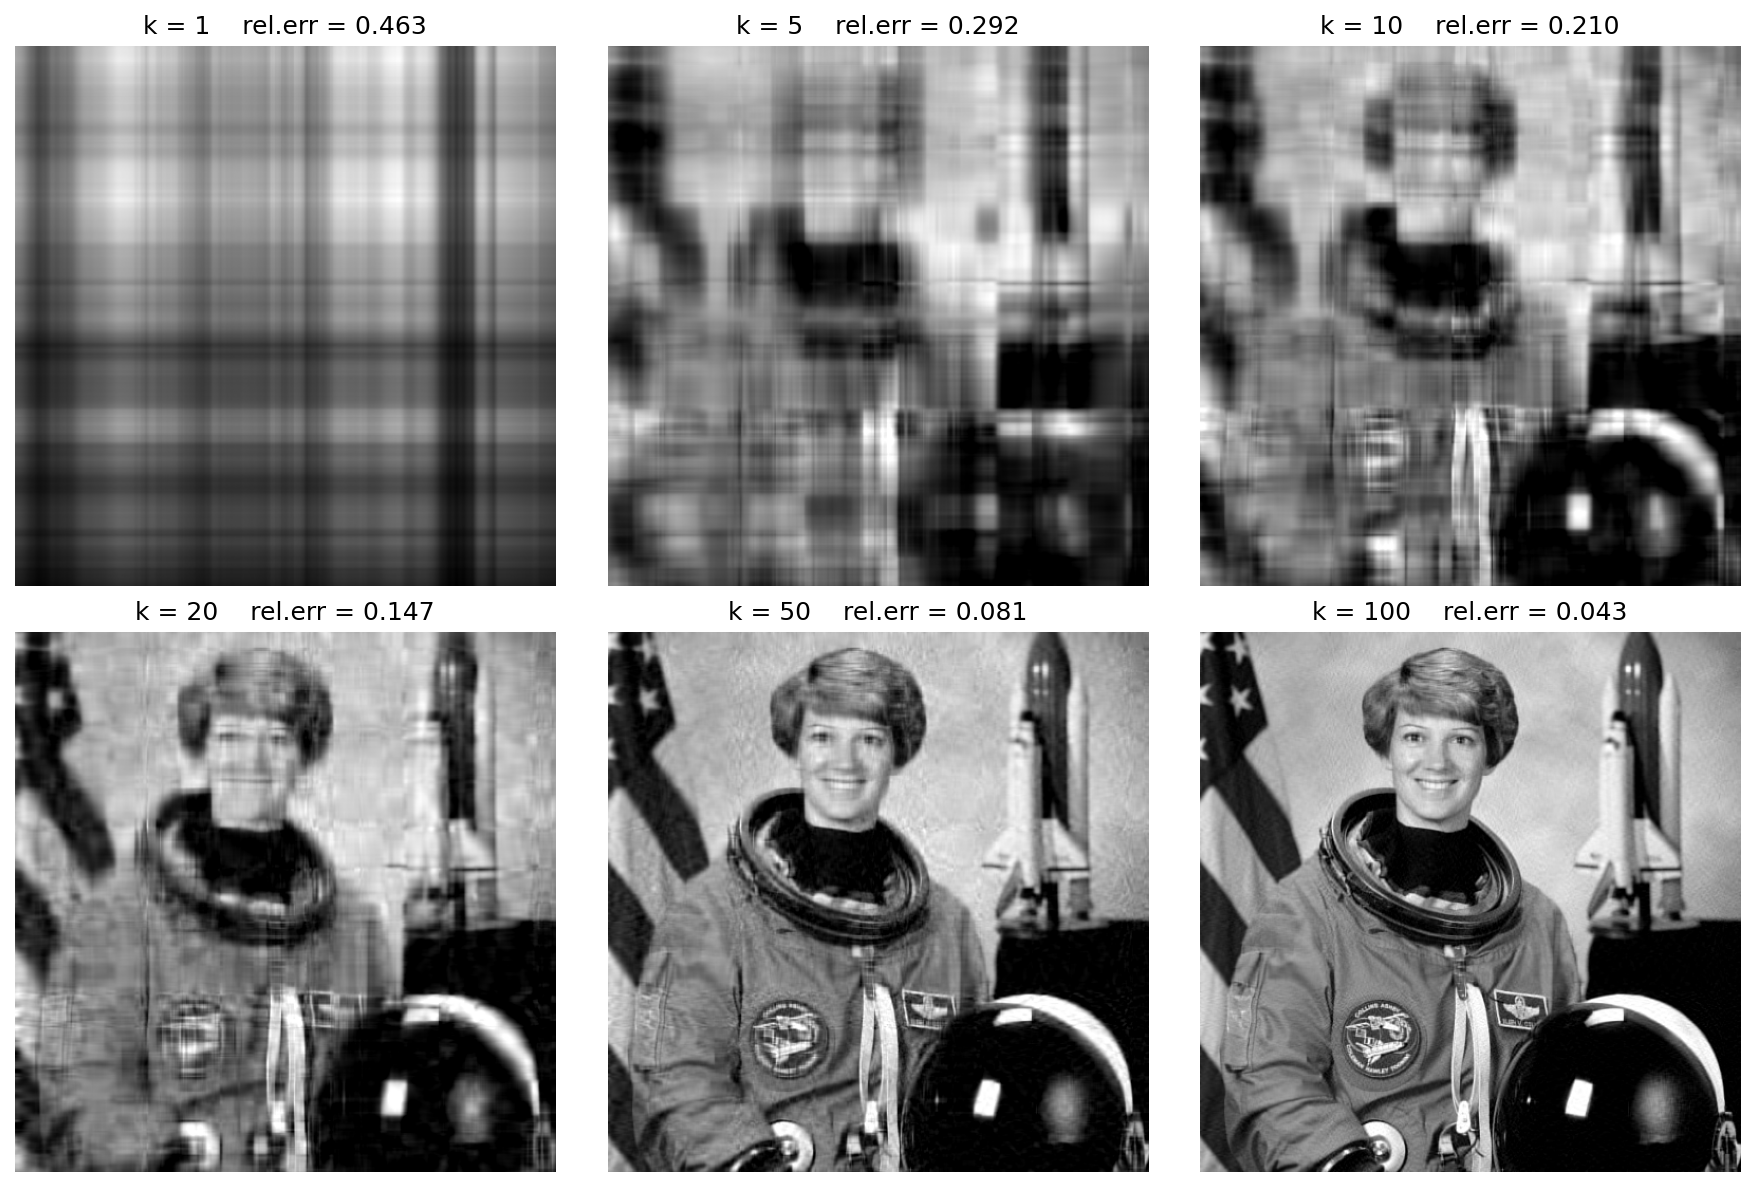
\includegraphics[width=\linewidth,height=0.65\textheight,keepaspectratio]{reconstructions.png}
  \end{center}
  \footnotesize \textbf{Observations.}
  \begin{itemize}
    \item $k=1$: pure stripes -- captures only the dominant brightness pattern.
    \item $k=20$: silhouette emerges; face is recognisable but blurry.
    \item $k=50$: visually faithful reproduction at $20\%$ of full rank.
    \item Error roughly halves with each doubling of $k$, mirroring the spectrum's decay.
  \end{itemize}
\end{frame}

\begin{frame}{Storage at Imperceptible Quality Loss}
  \begin{center}
    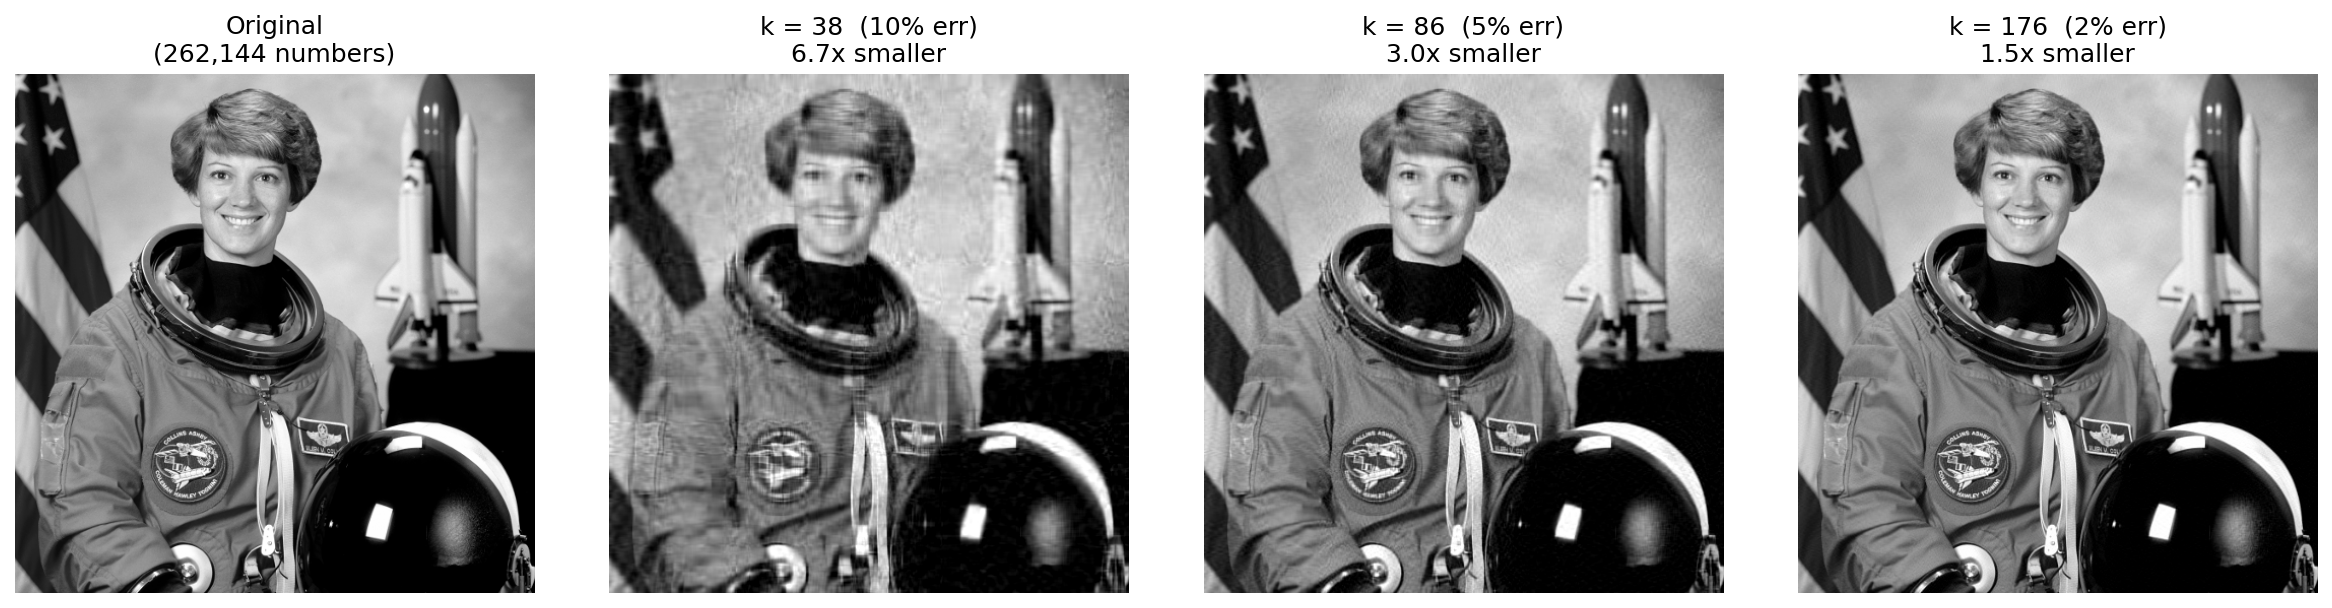
\includegraphics[width=\linewidth,height=0.65\textheight,keepaspectratio]{storage_demo.png}
  \end{center}
  \footnotesize \textbf{Observation.} At $10\%$ relative error: \textbf{6.7$\times$ compression}, visually nearly indistinguishable from the original. Tightening the target to $5\%$ costs us compression (only $3\times$); $2\%$ collapses to $1.5\times$. The trade-off is steep -- reaching the last few percent of fidelity is expensive.
\end{frame}

\begin{frame}{Denoising: Where Low-Rank Wins}
  \begin{columns}[T]
    \begin{column}{0.55\linewidth}
      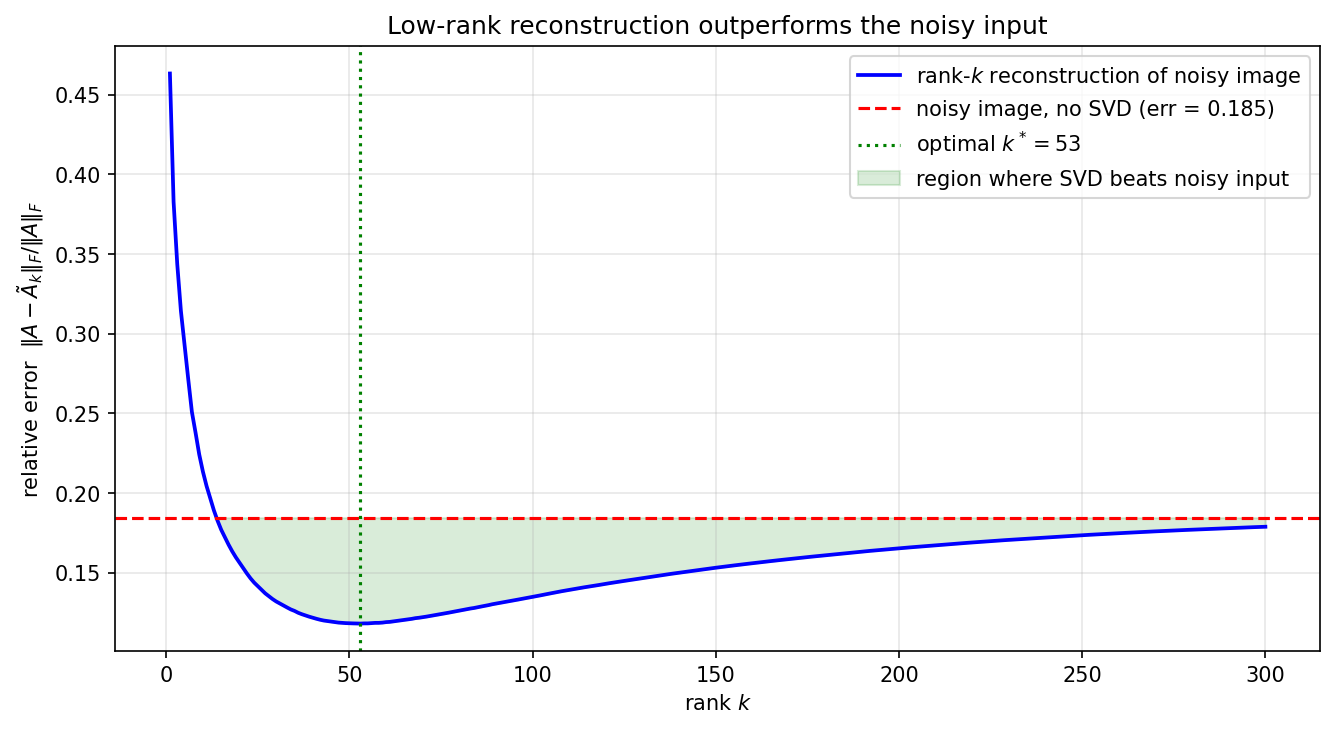
\includegraphics[width=\linewidth]{denoising_curve.png}
    \end{column}
    \begin{column}{0.42\linewidth}
      \footnotesize
      \textbf{Observations.}
      \begin{itemize}
        \item Noisy input: $\mathrm{err} = 0.185$.
        \item Optimal $k^* = 53$: $\mathrm{err} = 0.118$ -- a \textbf{36\% improvement} over keeping the noisy image.
        \item U-shape: too few components miss real signal; too many refit noise. This is the \emph{bias--variance trade-off} with rank as the complexity knob.
        \item The green region marks all $k$ where SVD beats doing nothing -- a wide window, not a knife-edge.
      \end{itemize}
    \end{column}
  \end{columns}
\end{frame}

\begin{frame}{Denoising: Visual}
  \begin{center}
    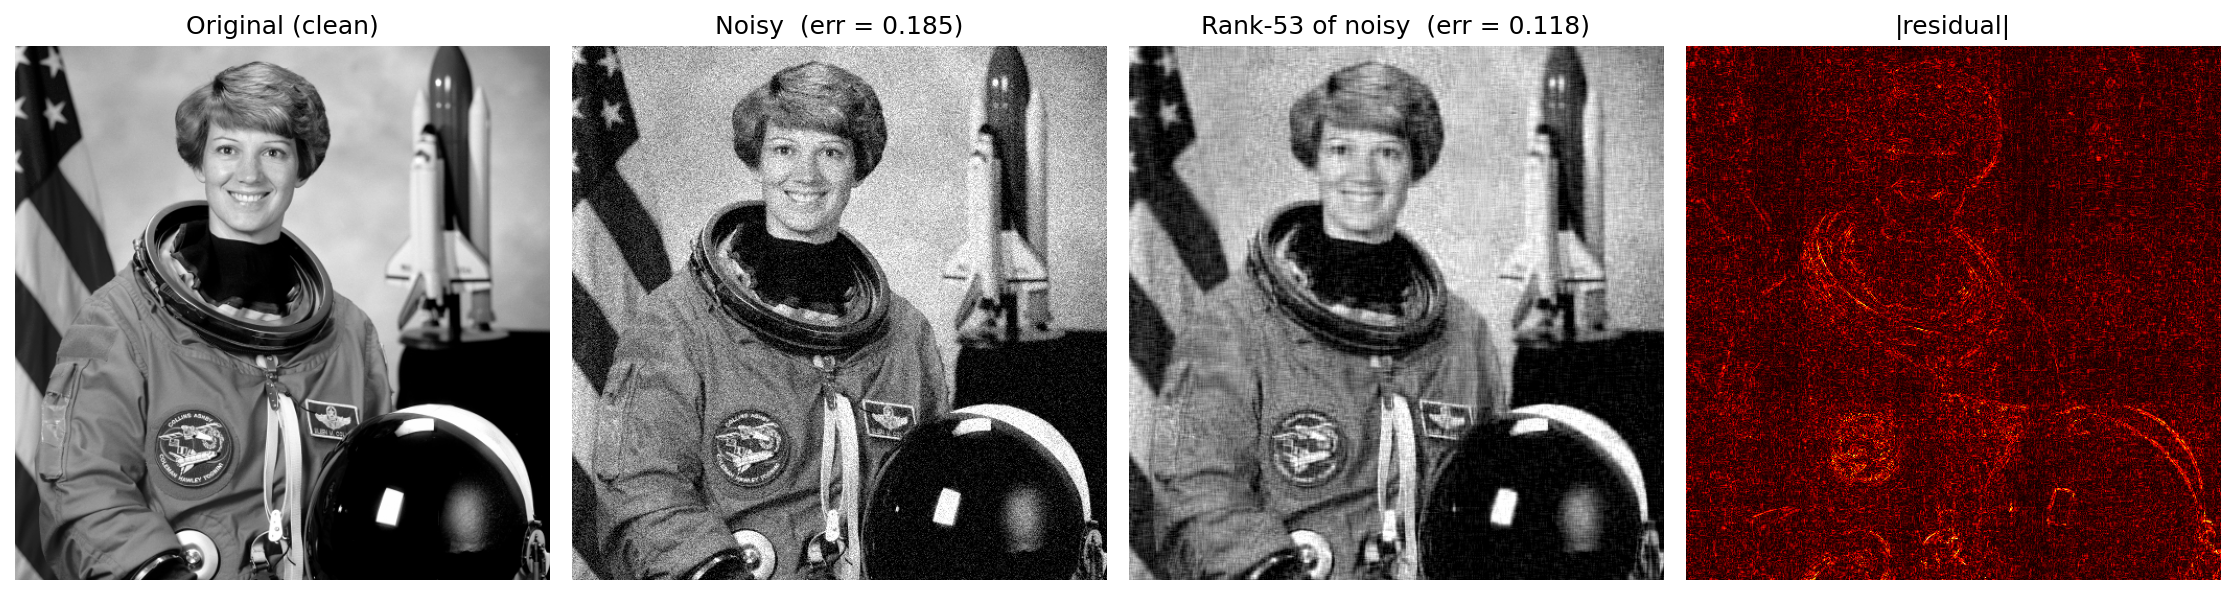
\includegraphics[width=\linewidth,height=0.65\textheight,keepaspectratio]{denoising_visual.png}
  \end{center}
  \footnotesize \textbf{Observations.} Noise concentrates in small singular values; truncation removes it. The residual map (rightmost) localises on edges, hair, and fine texture -- exactly where high-frequency content lives -- confirming that what we discard \emph{is} mostly noise plus genuine fine detail.
\end{frame}

\begin{frame}{Interactive Demo}
  Companion Streamlit app:
  \begin{itemize}
    \item Upload any image.
    \item Slider for rank $k$.
    \item Live: reconstructed image, error curve, storage ratio.
  \end{itemize}
  Run with: \quad \texttt{https://nla-image-compression-app.streamlit.app/}
\end{frame}

% =====================================================================
\section{Application 2: PCA on MNIST}
% =====================================================================

\begin{frame}{From SVD to PCA}
  Given centered data $X \in \R^{n \times d}$ ($n$ samples, $d$ features):
  \begin{itemize}
    \item Sample covariance: $C = \dfrac{1}{n-1} X^\top X$.
    \item SVD: $X = U \Sigma V^\top$.
    \item Principal directions: columns of $V$ -- eigenvectors of $C$.
    \item Variance along $v_i$: $\dfrac{\sigma_i^2}{n-1}$.
    \item Projection onto top $k$: $X_k = X V_k = U_k \Sigma_k$ (an $n\times k$ score matrix).
  \end{itemize}
  PCA $=$ SVD applied to centered data. The singular vectors are the principal axes; the singular values quantify how much variance lives along each.
\end{frame}

\begin{frame}{MNIST Setup}
  \begin{itemize}
    \item $28 \times 28$ digit images, flattened into $\R^{784}$.
    \item Centre: subtract the mean image.
    \item Compute SVD of the data matrix.
    \item Visualise:
      \begin{itemize}
        \item cumulative explained variance,
        \item 2-D scatter of top-2 PCs (coloured by digit class),
        \item ``eigendigits'' = leading right singular vectors reshaped to $28 \times 28$,
        \item reconstructed digits at $k = 5, 20, 50, 100$.
      \end{itemize}
    \item \textbf{Empirical result.} Top 50 components capture $\sim$$83\%$ of variance; top 100 capture $\sim$$92\%$. PCA features at $k=50$ achieve the same classification accuracy as the full $784$-pixel input, while training $\sim$$10\times$ faster.
  \end{itemize}
\end{frame}

\begin{frame}{Interactive Demo}
  Companion Streamlit app:
  \begin{itemize}
    \item Choose digit subset.
    \item Slider for number of components.
    \item Live 2-D / 3-D scatter, eigendigit gallery, on-the-fly reconstruction.
  \end{itemize}
  Run with: \quad \texttt{https://pca-mnist-app.streamlit.app/}
\end{frame}

% =====================================================================
\section{Conclusion}
% =====================================================================

\begin{frame}{Limitations \& What We Did Not Do}
  Honesty about scope:
  \begin{itemize}
    \item \textbf{Cost.} A full SVD costs $O(\min(mn^2, m^2 n))$. For very large matrices, randomised SVD or iterative Krylov methods are preferred -- we used the dense LAPACK routines via NumPy.
    \item \textbf{Norms.} Eckart--Young--Mirsky is optimal in $\norm{\cdot}_F$ and $\norm{\cdot}_2$, but \emph{not} in $\ell_1$ or $\ell_\infty$. Robust low-rank methods (e.g.\ robust PCA) tackle that case.
    \item \textbf{Compression vs.\ JPEG.} For natural images, JPEG and wavelets beat SVD because they exploit \emph{local} pixel correlations; SVD only captures global structure.
    \item \textbf{Choice of $k$.} We treated $k$ as a tunable knob. Data-driven optimal selection (Gavish--Donoho threshold, scree-elbow, cross-validation) is its own subject.
    \item \textbf{Streaming / out-of-core.} We assume the full matrix fits in memory. Online and incremental SVD algorithms exist for the streaming case.
  \end{itemize}
\end{frame}

\begin{frame}{Tooling}
  Built artefacts and libraries used:
  \begin{itemize}
    \item \textbf{Notebooks.} Jupyter, NumPy, Matplotlib, scikit-image, scikit-learn -- all theory checks and figures.
    \item \textbf{Streamlit apps.} Live, public, browser-based demos -- one per application.
    \item \textbf{This deck.} \LaTeX{} Beamer with the \texttt{metropolis} theme; diagrams in TikZ + pgfplots.
    \item \textbf{Source / live demos.}
      \begin{itemize}
        \item Image compression: \texttt{https://nla-image-compression-app.streamlit.app/}
        \item PCA on MNIST: \texttt{https://pca-mnist-app.streamlit.app/}
      \end{itemize}
  \end{itemize}
\end{frame}

\begin{frame}{Summary}
  \begin{itemize}
    \item \textbf{SVD} is the canonical decomposition exposing geometric and spectral structure of any matrix.
    \item \textbf{Frobenius and spectral norms} are unitarily invariant -- they depend only on the singular values.
    \item \textbf{Truncated SVD} is the optimal low-rank approximation in both norms (Eckart--Young--Mirsky), with closed-form error.
    \item \textbf{Rapid singular value decay} -- ubiquitous in real-world data -- is what makes compression and dimensionality reduction effective.
    \item Demonstrated on \textbf{image compression} (6.7$\times$ at imperceptible loss; 36\% denoising improvement) and \textbf{PCA on MNIST} (50 features match 784 pixels at $10\times$ speedup).
  \end{itemize}
\end{frame}


\begin{frame}{References}
  \footnotesize
  \begin{itemize}
    \item Trefethen \& Bau, \emph{Numerical Linear Algebra}, SIAM, 1997.
    \item Golub \& Van Loan, \emph{Matrix Computations}, 4th ed., JHU Press, 2013.
    \item Eckart, C.\ \& Young, G.\ (1936). \emph{The approximation of one matrix by another of lower rank}, Psychometrika 1, 211--218.
    \item Mirsky, L.\ (1960). \emph{Symmetric gauge functions and unitarily invariant norms}, Quart.\ J.\ Math.\ 11, 50--59.
    \item Gavish, M.\ \& Donoho, D.\ (2014). \emph{The optimal hard threshold for singular values is $4/\sqrt{3}$}, IEEE Trans.\ Inf.\ Theory 60(8).
  \end{itemize}
\end{frame}

\begin{frame}
  \centering
  \vspace{1cm}
  {\Huge Thank you!}\\[1cm]
  {\Large Questions?}
\end{frame}

\end{document}